\chapter{Deep Learning}
\section*{Infrastructure}
Model Architecture: UNET 2D and 3D

Trained on A100 GPU 80 GB using Maxwell Cluster at DESY. 

\section{Results}

\begin{figure}
    \centering
    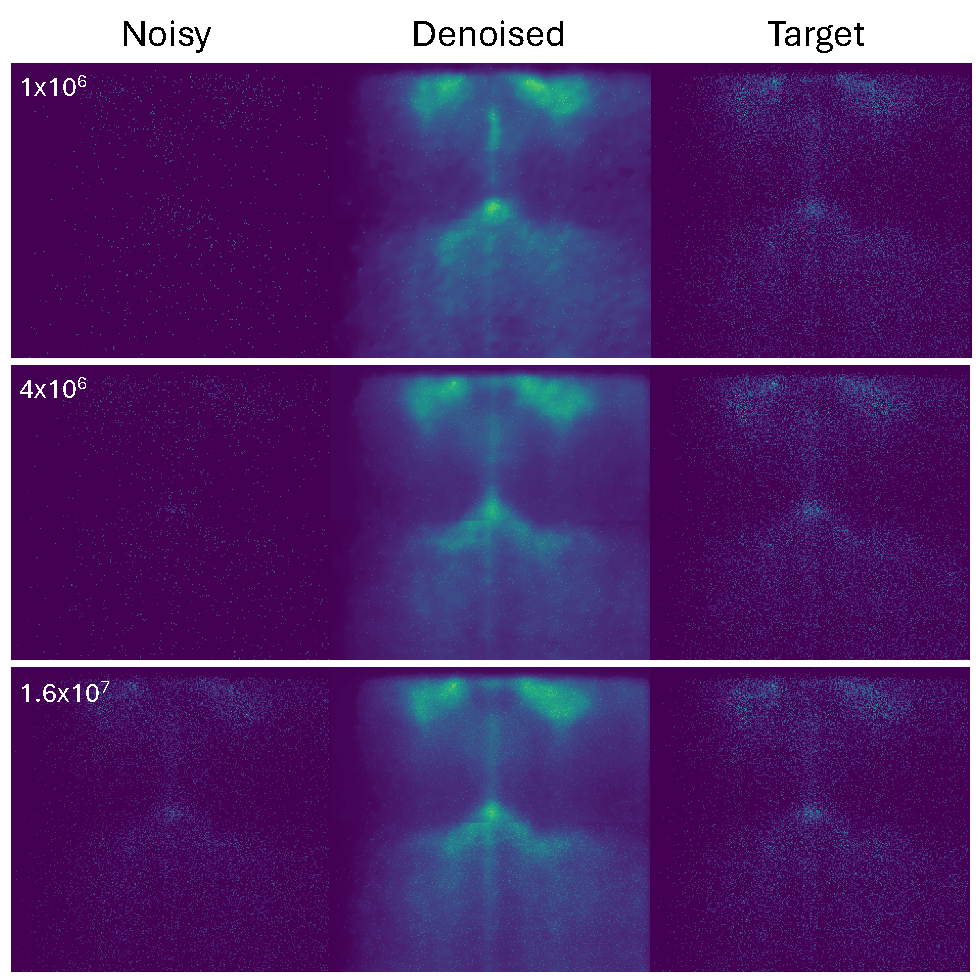
\includegraphics[width=1\linewidth]{images/nn_denoised_ex_single_slice.pdf}
    \caption{Noisy, denoised, and target \gls{E}-\gls{kx} cuts with window size $w=1$ shown for \gls{GdW} dataset. Each row corresponds \numlist{1e6;4e6;1.6e7} counts, respectively.}
    \label{fig:nn-denoised-ex-single-slice}
\end{figure}

\begin{figure}
    \centering
    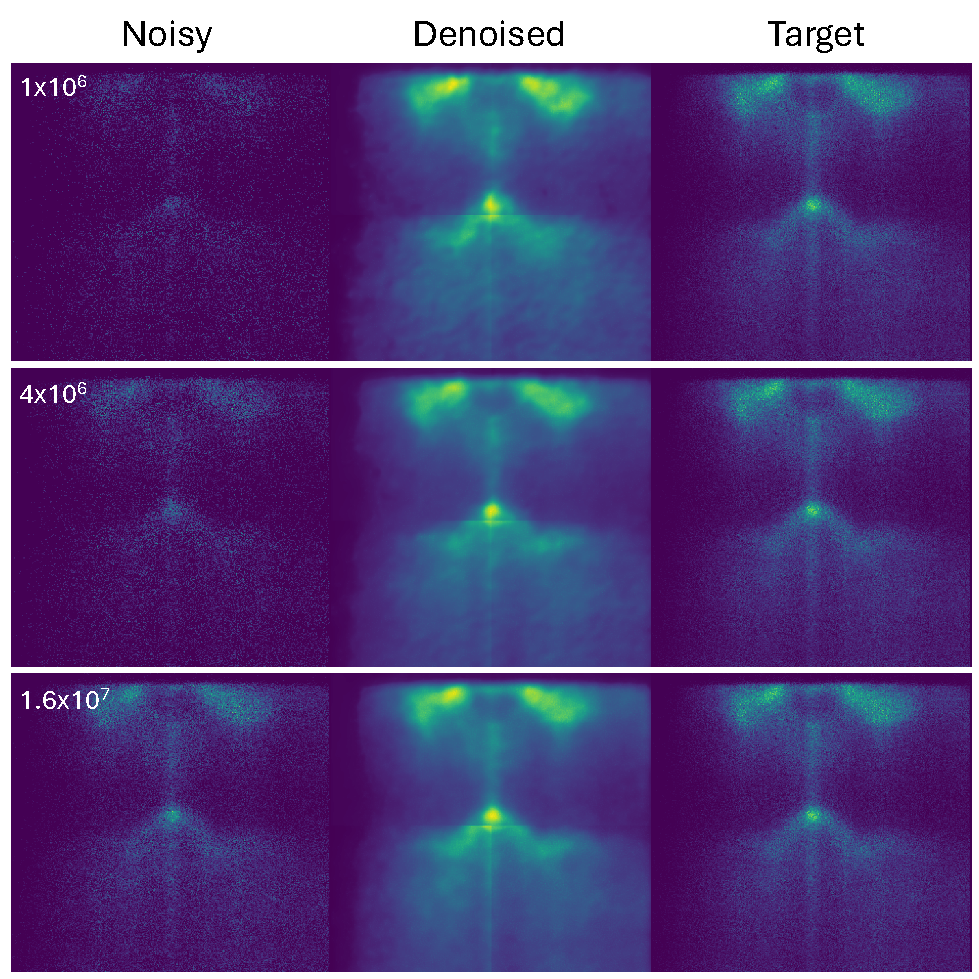
\includegraphics[width=1\linewidth]{images/nn_denoised_ex_20_slice.pdf}
    \caption{Noisy, denoised, and target \gls{E}-\gls{kx} cuts with window size $w=20$ shown for \gls{GdW} dataset. Each row corresponds \numlist{1e6;4e6;1.6e7} counts, respectively.}
    \label{fig:nn-denoised-ex-20-slice}
\end{figure}

\begin{figure}
    \centering
    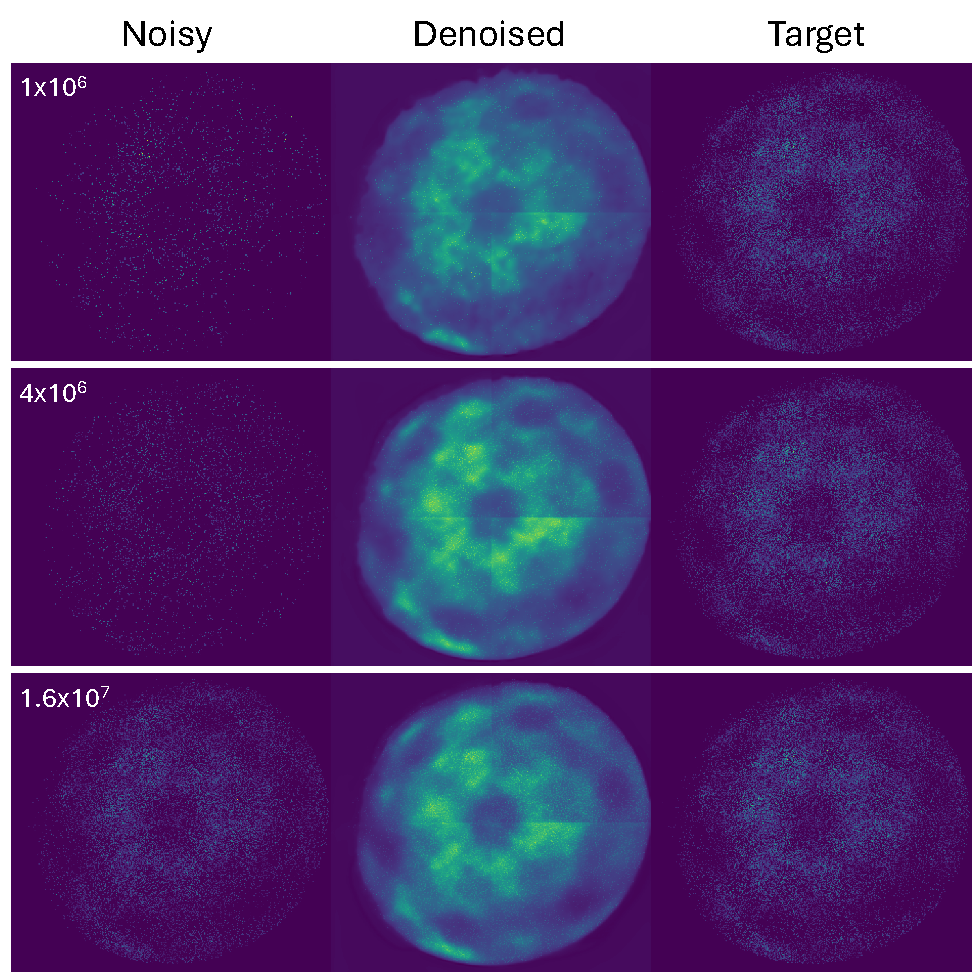
\includegraphics[width=1\linewidth]{images/nn_denoised_xy_single_slice.pdf}
    \caption{Noisy, denoised, and target \gls{ky}-\gls{kx} cuts with window size $w=1$ shown for \gls{GdW} dataset. Each row corresponds \numlist{1e6;4e6;1.6e7} counts, respectively.}
    \label{fig:nn-denoised-xy-single-slice}
\end{figure}

\begin{figure}
    \centering
    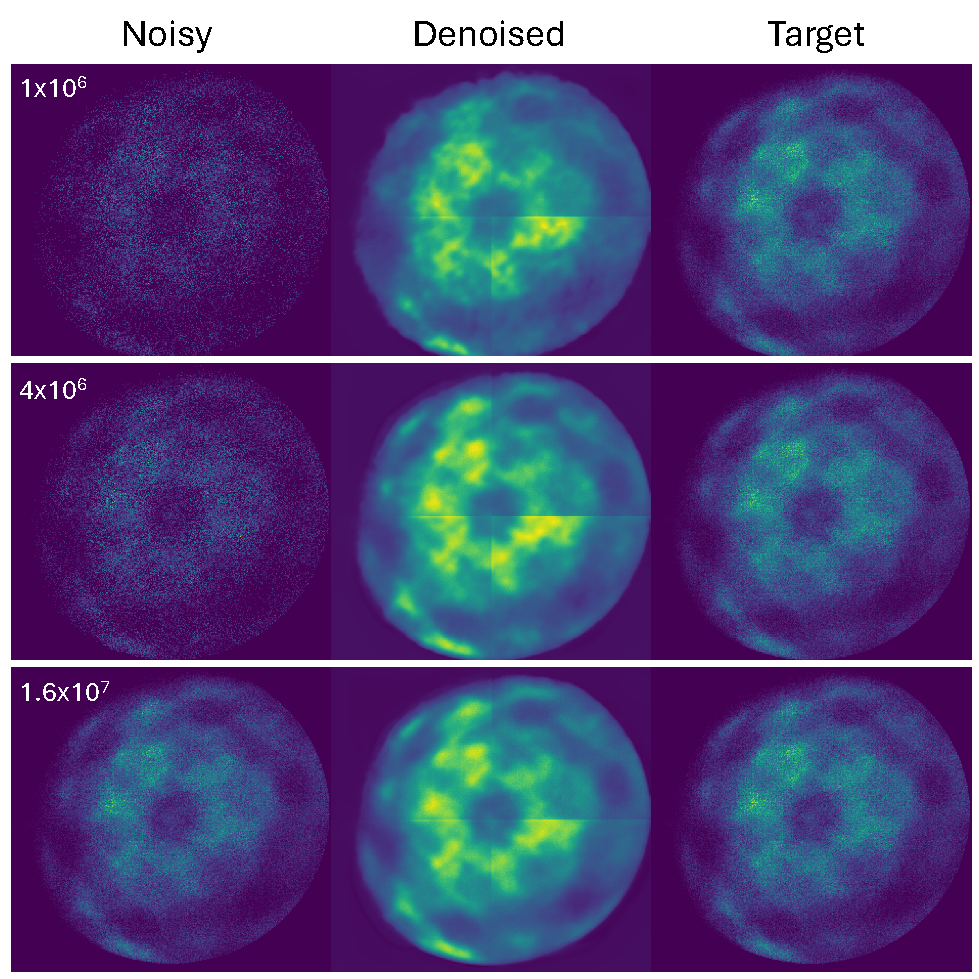
\includegraphics[width=1\linewidth]{images/nn_denoised_xy_20_slice.pdf}
    \caption{Noisy, denoised, and target \gls{ky}-\gls{kx} cuts with window size $w=20$ shown for \gls{GdW} dataset. Each row corresponds \numlist{1e6;4e6;1.6e7} counts, respectively.}
    \label{fig:nn-denoised-xy-20-slice}
\end{figure}